\chapter{Resultados} \label{resultado}

Neste capítulo são apresentados os resultados obtidos .

\section{Carga de Tração}

Utilizando de exemplo a manilha da Green Pin que possui WLL de 49 kN (5 toneladas), conforme anexo A e levando em consideração que o componente se equipara à utilização de 2 manilhas comerciais, temos o comparativo conforme  \ref{comparativo}. Indicando que o WLL encontrado é coerente.

\begin{table}[!ht]
\centering
\caption{Comparativo da relação WLL x peso do componente.}
\label{comparativo}
\begin{tabular}{ P{2.5cm} | P{3cm} | P{2.5cm} | P{2.5cm} | P{3cm} } 
\hline
\textbf{Componente} & \textbf{WLL (kN)} & \textbf{Peso por unidade (kg) } & \textbf{Peso do conjunto (kg) } & \textbf{Relação kN/kg} \\ \hline
 Green Pin & 49,0 & 0,63 & 1,26 & 38,88\\ 
\hline
 Proposta & 42,5 & 1,07 & 1,07 & 39,71\\ 
\hline
\end{tabular} \\
\smallskip
\hspace{1.5cm}\raggedright \fontsize{10}{12}\selectfont{Fonte: Elaborado pelo autor, 2025.}
\end{table}

As maiores tensões equivalentes aparecem próximo às áreas de contato, com a tensão máxima equivalente aparecendo na face de contato do carregamento no furo superior, como mostra a  \ref{finalequivalente2}, bem como os fatores de segurança associados, indicados na  \ref{fatorsegurancafinal}.



\begin{figure}[!htb]
   \centering
     \caption{Fator de segurança na geometria final.}
    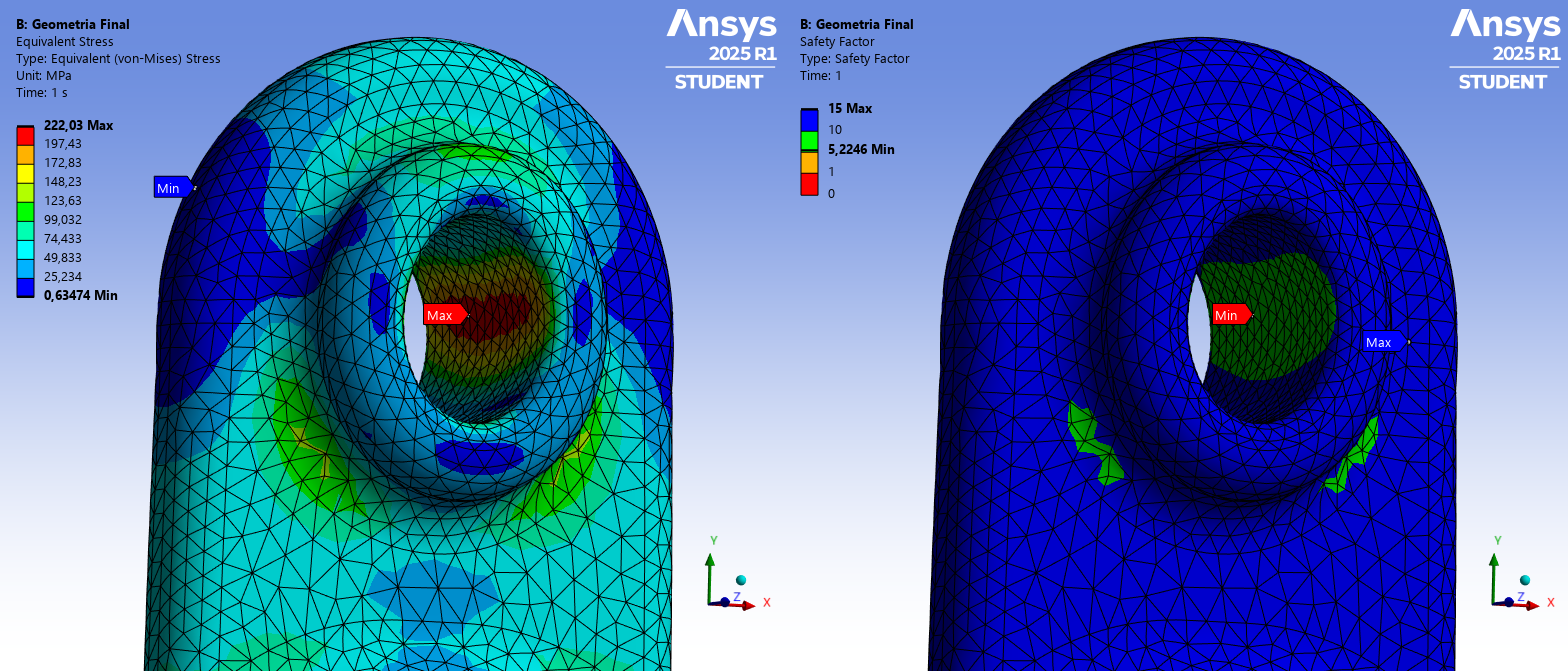
\includegraphics[width=1.0\linewidth, trim=0 0 0 0, clip]{Figuras/geometria final tensao equivalente 6.png}\\
    \hspace{1.5cm}\raggedright \fontsize{10}{12}\selectfont{Fonte: Elaborado pelo autor, 2025.}
    \label{fatorsegurancafinal}
\end{figure}

A título de comparação, a carga de trabalho de 42,5 kN foi aplicada na geometria inicial. Os resultados mostram uma tensão equivalente de Von Misses de 405,04 MPa e um fator de segurança mínimo de 2,86:1, indicando uma perda de 46 \% de capacidade para uma mesma carga de trabalho, como mostra a  \ref{fatorsegurancainicial}.

\begin{figure}[!htb]
   \centering
     \caption{Fator de segurança na geometria inicial.}
    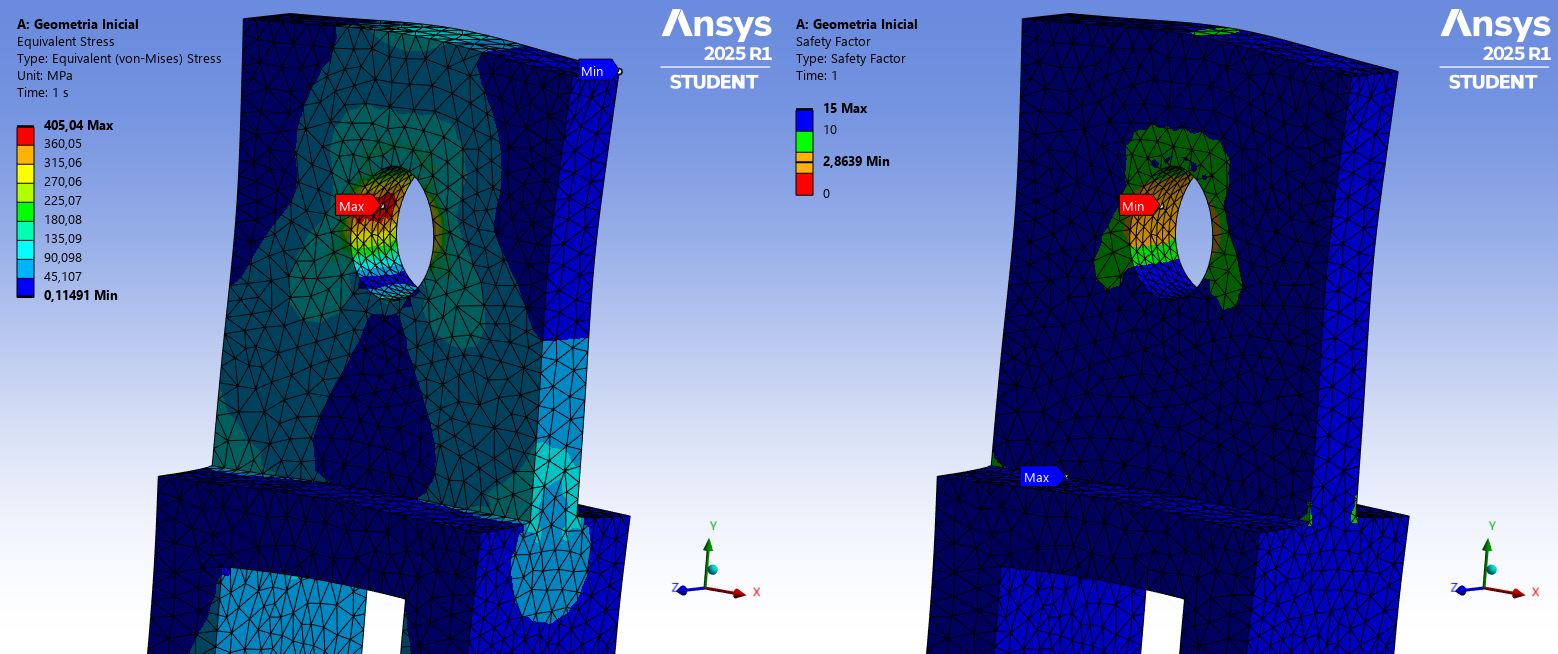
\includegraphics[width=1.0\linewidth, trim=0 0 0 0, clip]{Figuras/geometria inicial tensao equivalente 5.png}\\
    \hspace{1.5cm}\raggedright \fontsize{10}{12}\selectfont{Fonte: Elaborado pelo autor, 2025.}
    \label{fatorsegurancainicial}
\end{figure}


